\section{Member 3: Gaussian classifiers}
\label{sec:m3}
\textbf{Code:} \code{models/gaussian.py}, \code{experiments/c2\_gaussian.py}.

\paragraph{The models.}
Each class is modelled as a multivariate Gaussian, and Bayes' rule gives $\post$. The \emph{shared}
model pools one covariance matrix for both classes, which gives a linear boundary; the
\emph{class-specific} model fits one per class, which gives a quadratic one. On Spambase many features
are almost always zero within a class, so the raw covariances are singular. We shrink them towards a
multiple of the identity, $S\mapsto(1-\alpha)S+\alpha\,\tfrac{\operatorname{tr}S}{d}I$, with $\alpha$
chosen on validation log-loss. All densities are computed in the log domain from Cholesky factors,
without inverting any matrix. The tests show the shared model agrees with scikit-learn's LDA to
$10^{-8}$ and the class-specific model with its QDA to $10^{-6}$.

\paragraph{Does $\log(1+x)$ help?}
Word counts are far from Gaussian. The script compares plain standardisation with $\log(1+x)$ followed
by standardisation, over the 20 splits (Table~\ref{tab:c2}).

\begin{table}[!htbp]
\centering\footnotesize\setlength{\tabcolsep}{4pt}
\input{\resultsdir/c2_gaussian_summary.tex}
\caption{Gaussian classifiers on Spambase, test mean $\pm$ standard error over 20 splits. $\alpha$:
chosen shrinkage (median). Accuracy uses the cut $0.5$; ``Loss $\tstar$'' is the cost of the
two-action rule and ``Loss Bayes'' that of the rule with inspection ($\cfp=10$, $\cfn=1$, $\ci=0.3$).}
\label{tab:c2}
\end{table}

\begin{figure}[!htbp]
\centering
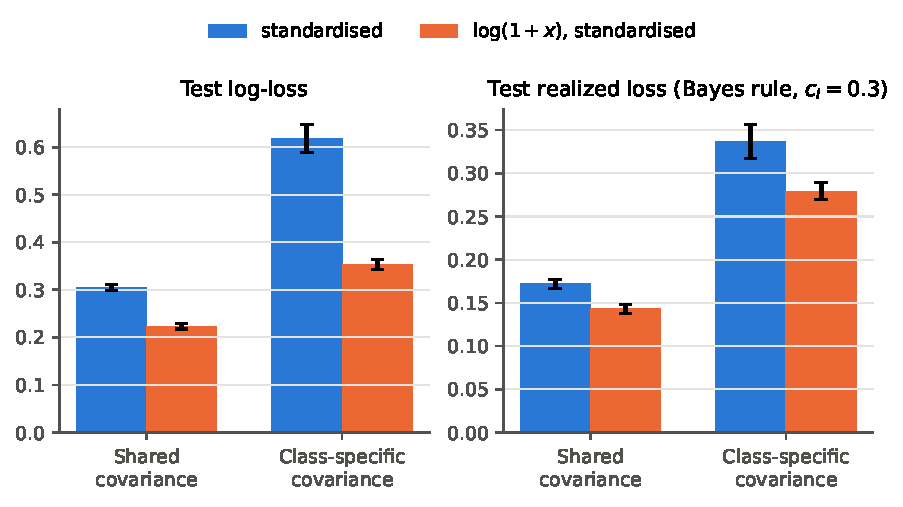
\includegraphics[width=0.8\linewidth]{c2_gaussian_log1p.pdf}
\caption{Spambase: test log-loss and realized loss of the two Gaussian models with and without
$\log(1+x)$ (mean $\pm$ standard error over 20 splits).}
\label{fig:c2}
\end{figure}

The transform helps both models (Figure~\ref{fig:c2}). For the shared model the test log-loss falls from $0.305$ to
$0.223$ and the cost with inspection from $0.172$ to $0.143$. The class-specific model stays far worse
with either preprocessing: each class needs its own $57\times57$ covariance, validation chooses heavy
shrinkage ($\alpha\approx0.9$), and $2{,}761$ training emails are not enough to pay for the extra
flexibility. Members 1 and 5 therefore use the shared model with $\log(1+x)$ features.
